\documentclass{article}

\usepackage{arxiv}

\usepackage[utf8]{inputenc} % allow utf-8 input
\usepackage[T1]{fontenc}    % use 8-bit T1 fonts
\usepackage{hyperref}       % hyperlinks
\usepackage{url}            % simple URL typesetting
\usepackage{booktabs}       % professional-quality tables
\usepackage{amsfonts}       % blackboard math symbols
\usepackage{amsmath}        % equations
\usepackage{nicefrac}       % compact symbols for 1/2, etc.
\usepackage{microtype}      % microtypography
\usepackage{graphicx}
\usepackage[numbers]{natbib}
\usepackage{doi}

\title{Evidence of fault zone transport of road-salt contaminated groundwater from highways to streams}

% TODO: The source docx contains no author block. Names below are from the
% project record (senior honors thesis at Marist); fill in departments,
% emails, and ORCIDs before submission.
\author{
	Tadd Bindas \\
	\texttt{taddbindas@gmail.com} \\
	\And
	Zion Klos \\
	Marist University\\
	Poughkeepsie, NY \\
	\texttt{zion.klos@marist.edu} \\
}

\date{}

\renewcommand{\shorttitle}{Fault zone transport of road-salt contaminated groundwater}

\hypersetup{
pdftitle={Evidence of fault zone transport of road-salt contaminated groundwater from highways to streams},
pdfauthor={Tadd Bindas, Zion Klos},
pdfkeywords={water quality, fault lines, salinity, de-icing, roadway management},
}

\begin{document}
\maketitle

\begin{abstract}
Many streams in the northeastern U.S. have seen increased salinity in recent decades, correlating with the surge in use of salt as a deicing agent on roads. These rises in freshwater salinity have led to decreases in water quality and impaired ecological health. Instead of seeing stream salinity levels decline during summer months, when there is a negligible application of salt, levels of salinity often rise during these periods of baseflow. This increase corresponds to the time of year when the proportional contribution of groundwater input to overall streamflow is at its peak. We suspect there is a spatial correlation between the location of where these salt inputs occur, causing rises in late summer stream salinity, and the heterogeneous locations of geologic fault zones, which could preferentially move groundwater rapidly, and under topographic divides, from highway to stream -- a phenomenon observed by others, but only in groundwater wells. After detailed spatial surveys of key locations of Wappingers Creek in Dutchess County, NY, we determined that of the three clear fault zone crossings not confounded by a corresponding tributary in the same location, two showed statistically significant increases ($\alpha$ = 0.05) in specific conductance at the fault locations. Our findings suggest most similar fault zones mapped throughout the region may possess the potential to facilitate preferential transportation of high salinity groundwater from roadways into streams, even from kilometers away, demonstrating the need to incorporate currently mapped fault zones into considerations of both roadway and water quality management plans.
\end{abstract}

\keywords{water quality \and fault lines \and salinity \and de-icing \and roadway management}

\section{Introduction}

Road salt is indispensable for winter road safety, yet it introduces a widespread salinization threat to fresh waters across cold-climate regions \citep{kaushal2005,dugan2023}. Introduced in the early 1940s as a road de-icing agent in North America and Europe, road salt's usage has climbed steadily decade over decade \citep{tiwari2018,bubeck1971,jackson2005}. However, this tool is effective only within a temperature window; below roughly $-9.5$~$^{\circ}$C (15~$^{\circ}$F) salt becomes marginally effective, melting demands very high application rates, and most transportation agencies advise against its use \citep{kelting2010}. In practice, it is nonetheless applied under these conditions and in amounts beyond what de-icing requires, leading to long-term impacts on infrastructure, cars, groundwater, ecosystems, and wildlife \citep{jamshidi2020,findlay2011}. Structurally, road salts have corrosive effects which accelerate damage to both automobiles and bridges \citep{kelting2010}. Environmentally, road salts have been shown to contaminate groundwater and decrease stream water quality \citep{jackson2005,williams1999} while persisting in soil for a minimum of 2.5--5 months \citep{robinson2017}. Furthermore, adverse environmental effects of road salt use include salt-tolerant invasive species outbreaks \citep{richburg2001}, disruption of roadside and aquatic habitat \citep{forman1998}, and shifts in algal communities toward cyanobacterial (blue-green algae) dominance as salinity rises \citep{dugan2023}. Despite the application of road salts only occurring during months where temperatures approach or are below freezing, side effects of their application exist during all months of the year \citep{shattuck2023}.

These accumulating impacts are increasingly understood not as isolated effects but as facets of a single systemic process. \citet{kaushal2018} termed the concurrent, long-term rise in salinity, alkalinity, and associated major ions across fresh waters the ``freshwater salinization syndrome,'' documenting its progression across the contiguous United States. Subsequent work reframes salinization as a global biogeochemical disturbance: \citet{kaushal2023saltcycle} describe an ``anthropogenic salt cycle'' in which human activities accelerate the mobilization, storage, and delayed release of salts among soil, water, and air. Most relevant to the present study, \citet{kaushal2023factors} identify five state factors that govern the severity and trajectory of the syndrome: human activity, geology, flowpaths, climate, and time. This framework explicitly names subsurface geology and hydrologic flowpaths as first-order controls on where and how salt reaches streams. This framing motivates a search for the specific geologic structures and flowpaths that concentrate the delivery of stored salt to surface water.

The ecological and management stakes of freshwater salinization are substantial. Road deicing salt is released almost entirely into the environment and is a widespread pollutant of freshwater lakes, rivers, wetlands, and groundwater in cold-climate regions \citep{dugan2023}. Its effects propagate through aquatic food webs via osmoregulatory stress and community-level feedbacks, and they occur at chloride concentrations at or below existing regulatory guidelines: in a coordinated experiment spanning lakes in North America and Europe, \citet{hintz2022} found that chloride levels at or beneath current water-quality thresholds caused substantial losses of zooplankton and, at nearly half of the study sites, cascading increases in phytoplankton. Because present guidelines do not reliably protect freshwater ecosystems, identifying \emph{where} salt enters streams, and therefore where mitigation would be most effective, carries direct management value.

While it has been shown that chloride concentrations are highest in the winter \citep{corsi2015}, a lag-effect of higher salinity concentrations in the summer months has been linked to road salt application \citep{kelly2008}. When stream discharge is low during the summer months, groundwater inputs keep many perennial streams flowing at baseflow. As road salts continue to infiltrate into groundwater over recent decades \citep{rivett2016}, summer time stream salt concentrations continue to rise through surface-groundwater exchange, leading to examples of long-term salinity increases globally \citep{williams1999,kaushal2005,foos2003}. This baseflow signal reflects a growing legacy of salt stored in the subsurface: mass-balance studies in salted regions show that much of the applied chloride does not flush through quickly but accumulates in groundwater, from which it is released to streams over years to decades \citep{vanmeter2024}, so that summer baseflow salinity integrates decades of past application rather than the most recent winter alone.

If a stream's summer baseflow salinity reflects salt stored in and slowly released from groundwater, then the subsurface geologic structure routing that groundwater should govern where along the channel the stored salt re-emerges \citep{kaushal2023factors}. The clearest evidence to date comes from bedrock wells: \citet{schalk2012} documented four road-salt-contaminated wells along a fault zone in Maine with elevated specific conductance in both summer and winter, traced to a roadway running along the fault's trace. Faults are more generally recognized as preferential water flow paths \citep{bredehoeft1992,gudmundsson2000}, and specifically as conduit-barrier systems \citep{bense2008}. Yet direct evidence that faults deliver highway road salt to streams remains scarce, leaving open whether these structures act as conduits routing contaminated groundwater to surface water. Resolving this has practical stakes: it would flag streams that are geologically connected to a highway through a fault, and thus at risk, even where no road runs nearby.

If faults do route contaminated groundwater to streams, the expectation is specific and spatially testable. Where a conductive fault crosses a channel, salt-laden groundwater discharging along the structure should produce an abrupt, localized rise in specific conductance between the reaches immediately upstream and downstream of the crossing, rather than the gradual downstream drift expected from diffuse inputs. That step should persist into summer baseflow, when direct runoff is absent and streamflow is dominated by groundwater, and it should be reflected in chloride, the ion that most directly fingerprints deicing salt. A dense longitudinal survey of specific conductance, paired with mapped fault traces and a targeted chloride transect, provides exactly this test, and is the approach we take here.

Here, we present a case study of Wappinger Creek in Dutchess County, New York, testing whether sharp increases in stream salinity coincide spatially with mapped high-angle faults, as an example of fault-conduit transport of road-salt-contaminated groundwater from highway to stream. We focused on stream reaches where previously mapped high-angle faults are oriented to route groundwater preferentially from major highways to nearby streams, potentially over kilometers of distance and beneath topographic divides.

\section{Methods}

\subsection{Site description}

For our study we selected three segments of Wappinger Creek, a tributary to the Hudson River in Dutchess County, New York, USA. Each site was chosen based on two factors: whether one or more high-angle faults intersect the stream, and whether the segment could be accessed safely. A geologic fault-line map of Dutchess County \citep{budnik2010} allowed us to locate each stream intersection with a high-angle fault and to create a detailed map (Figure~\ref{fig:overview}) containing both fault lines and major roads. Wappinger Creek intersects State Highways 44, 55, and 9, as well as the Taconic State Parkway, in various sections. Multiple faults bisect the creek in its upper east fork and its middle section, and the traces of some of these structures appear to control the channel's course, most visibly at Sites 1 and 2.

The bedrock beneath the study area consists of metamorphosed clastic sedimentary rocks that were folded and faulted during the Taconic Orogeny, and it is cut by low-angle thrust faults as well as steeper, high-angle faults \citep{budnik2010}. This structural setting is central to our hypothesis, because fault zones typically comprise a fractured, high-permeability damage zone flanking a lower-permeability core, and can therefore behave as preferential conduits, as barriers, or as combined conduit-barrier systems for groundwater flow \citep{bense2008,gudmundsson2000}. Where the damage zone is well connected, faults can transmit groundwater rapidly and with strong directional anisotropy: at the Hidden Valley fault zone in central Texas, for instance, \citet{ferrill2025} used dye-tracer tests in the Cretaceous Glen Rose Formation (Trinity Aquifer) to document groundwater moving up to roughly 2{,}600~m/day parallel to the fault and about 990~m/day across the adjacent damage zone, yielding a bulk hydraulic conductivity more than seven times greater parallel to the fault than perpendicular to it. If the high-angle faults crossing Wappinger Creek behave comparably, they could route road-salt-laden groundwater from a highway to the channel even where the two are separated by a topographic divide, motivating our focus on stream reaches that coincide with mapped fault traces.

\begin{figure}[htbp]
	\centering
	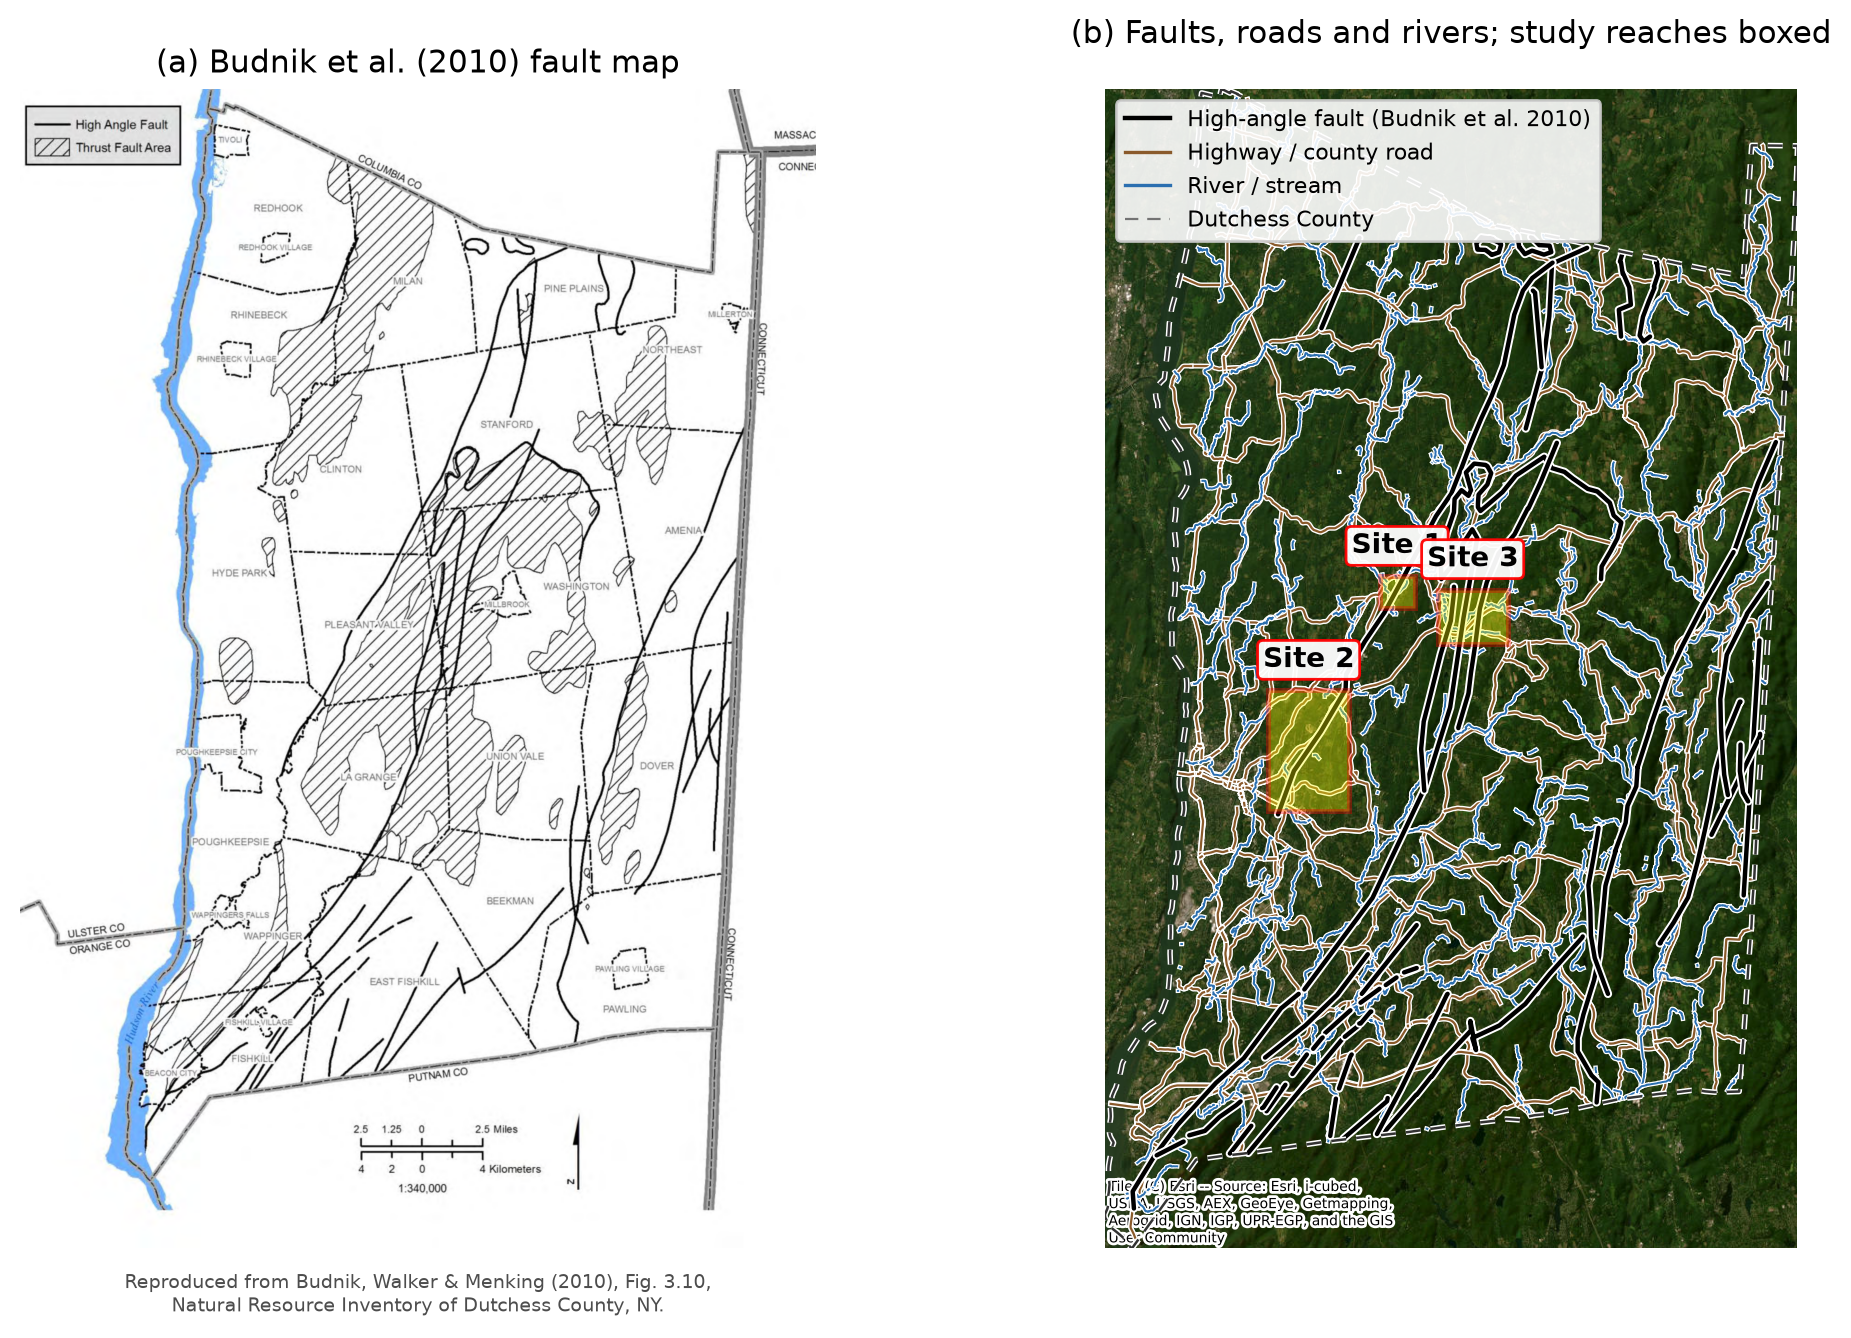
\includegraphics[width=\linewidth]{figures/overview.png}
	\caption{Study area overview. (a) The county fault map, taken directly from \citet{budnik2010}, Fig.~3.10, showing high-angle faults and thrust-fault areas across Dutchess County. (b) The three study reaches on Wappinger Creek (black boxes) on an OpenStreetMap base, with the same high-angle faults overlaid; each site sits where a high-angle fault crosses the creek. Reach-scale conductivity for each site is detailed in Figures~\ref{fig:site1}--\ref{fig:site3}.}
	\label{fig:overview}
\end{figure}

\subsection{In-situ sampling}

Conductivity measurements were obtained in October 2018; taking measurements approximately every hundred meters upstream to downstream traversing either on foot inside or around the creek or floating along the channel. Sampling was performed in the thalweg of each study site using an electrical conductivity (EC) meter logging the specific conductance of the water, through which we inferred changes in levels of salt input to the stream along its length.

Performing measurements in the thalweg kept our data objective by reducing potential variations due to lateral mixing. EC was converted to specific conductivity through adjusting the probe to 25 degrees Celsius. Measurements were taken using a Thermo Scientific Orion 013010MD Conductivity Cell calibrated using the standard protocols outlined by the manufacturer.

Each site was surveyed at a nominal spacing of roughly 100~m from upstream to downstream, yielding 9, 18, and 46 measurement points at Sites 1, 2, and 3, respectively, with point positions recorded using a handheld GPS unit. Within each site we delineated zones bounded at the locations where the creek crosses a mapped fault trace or receives an active tributary, so that the reaches immediately upstream and downstream of a single geologic or hydrologic feature could be compared directly. To isolate the effect of faults, we restricted our fault-crossing contrasts to reaches where the creek intersects a mapped fault without a coincident tributary, because a tributary confluence introduces an independent salinity signal that would confound the comparison. Because the fault traces are mapped at county scale \citep{budnik2010}, their horizontal positions carry an uncertainty of up to a few hundred meters; we therefore treated each crossing as a reach-scale rather than a point-scale feature when assigning zone boundaries. Zones are numbered such that they ascend as the river goes downstream: for example zone 3-3 is downstream of 3-2 which is downstream of 3-1. Comparable dense spatial surveys of specific conductance and chloride have been used elsewhere to trace groundwater-sourced road salt to streams and springs, including in a karstic watershed where springs showed the strongest long-term increases \citep{orr2026}.

Chloride was assessed electronically using a calibrated YSI multi-probe during July 2020 within Site 3, upstream and downstream of the long-term monitoring location of \citet{kelly2019}, to determine whether rises in chloride concentration occurred close to the mapped geologic faults. This longitudinal chloride transect spanned roughly one kilometer of the east fork, expressed as relative distance from an upstream point Z to a downstream point Z' (Figure~\ref{fig:chloride}), and was collected in summer, when the stream is at baseflow and any elevated chloride is more plausibly attributed to groundwater than to concurrent road-salt runoff. Sampling in July, nearly two years after the October 2018 conductivity survey, also provided an independent test of whether the same spatial pattern recurred across years and across a second, more salt-specific measurement.

\subsection{Statistical analysis}

The specific conductance was normalized within each site using mean/standard-deviation (z-score) normalization (Equation~\ref{eq:normalization}), with the sample mean $\overline{X}$ and sample standard deviation $\sigma_x$ computed separately for each site. This removes day-to-day differences in the overall conductivity level and streamflow between sampling dates and places all sites on a common, dimensionless scale so that the relative rise or fall across a feature can be compared regardless of a site's absolute salinity.

\begin{equation}
	\mu_{0} = \frac{x - \overline{X}}{\sigma_{x}}
	\label{eq:normalization}
\end{equation}

Next, we separated the specific-conductance samples into zones defined by where geologic interactions occur, that is, where the stream crosses either a fault or a side-stream. We then applied a two-sample Welch $t$-test (Equation~\ref{eq:ttest}) to evaluate the difference in mean specific conductance upstream and downstream of each feature. Unlike Student's pooled $t$-test, Welch's version does not assume equal variances between the two zones, and it remains reliable when the groups have both unequal variances and unequal sample sizes, as ours do; for these reasons it is recommended as the default two-sample test \citep{ruxton2006}.

\begin{equation}
	t = \frac{\overline{x}_{2} - \overline{x}_{1}}
	         {\sqrt{\dfrac{s_{1}^{2}}{n_{1}} + \dfrac{s_{2}^{2}}{n_{2}}}}
	\label{eq:ttest}
\end{equation}

Here $\overline{x}_{1}$ and $\overline{x}_{2}$ are the mean specific conductance of the upstream and downstream zones, $s_{1}$ and $s_{2}$ their standard deviations, and $n_{1}$ and $n_{2}$ their sample sizes. Applying a $t$-test to measurements collected sequentially along a channel warrants caution, because closely spaced samples are not strictly independent. We treated the measurements within a zone as approximate replicates of that reach's ambient salinity and tested only the difference in means between adjacent zones; because the within-zone scatter is small relative to the between-zone contrasts (Table~\ref{tab:ttest}), we interpret a significant contrast as a genuine step change across the intervening feature rather than an artifact of fine-scale autocorrelation. Site 3 was surveyed over two days owing to its length, but every zone-to-zone contrast was computed within a single day's data, and the per-site normalization (Equation~\ref{eq:normalization}) removes any offset in baseline conductivity between the two days, so the comparisons remain valid. We evaluated significance with two-tailed tests at $\alpha = 0.05$. Because our zone samples are modest in size and not guaranteed to be normally distributed, we accompanied every Welch test with a distribution-free Mann--Whitney $U$ test and regard a contrast as robust only where the two approaches agree, which guards against over-interpreting the smaller contrasts.

\section{Results}

\subsection{Contrasts}

Site 1 was split into two zones (Zone 1-1 and Zone 1-2), with a single contrast (Contrast A) used for analysis where Wappinger Creek abruptly veers along the mapped fault trace (Figure~\ref{fig:site1}). Before the fault interaction, the sample-mean specific conductance for Zone 1-1 was 259.9~$\mu$S/cm; after the fault, at Zone 1-2, it decreased slightly to 259.4~$\mu$S/cm. This slight decrease across the fault, however, coincided with an active tributary entering the creek at the same location, so the contrast at Site 1 cannot be attributed to the fault alone. Site 1 is instructive nonetheless: the channel veers to follow the mapped fault trace (Figure~\ref{fig:site1}), precisely the geometry in which a fault-conduit signal might be expected to appear, but the coincident tributary, together with a rain event during sampling that lowered specific conductance across this reach by 50--100~$\mu$S/cm relative to the other two sites, makes this crossing unsuitable for isolating the fault. We therefore exclude Contrast A from the set of clean fault crossings.

\begin{figure}[htbp]
	\centering
	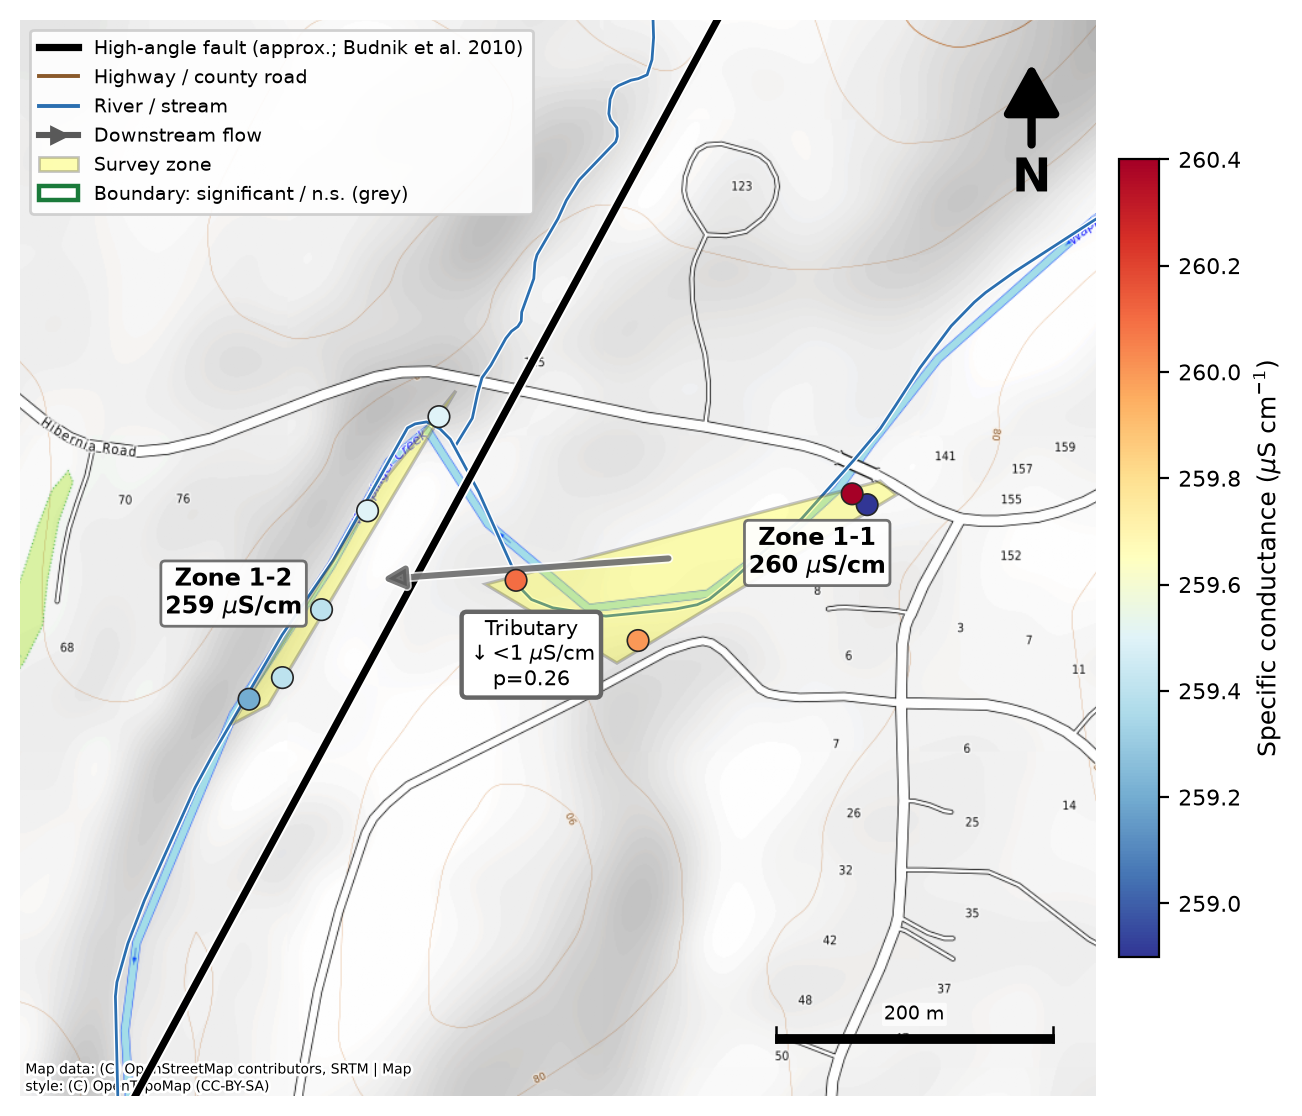
\includegraphics[width=0.62\linewidth]{figures/site1.png}
	\caption{Site 1 on a terrain base with highways/county roads (brown) and streams (blue). Survey points are coloured by specific conductance; red-outlined regions are the survey zones, labelled with their mean specific conductance. Zones are numbered in ascending order downstream (Zone 1-1 upstream, 1-2 downstream). High-angle faults (thick black lines) are approximate, digitized from \citet{budnik2010}. Statistical comparisons between zones are given in Table~\ref{tab:ttest}.}
	\label{fig:site1}
\end{figure}

Site 2 (Figure~\ref{fig:site2}) has one contrast (Contrast B) between two zones (Zones 2-1 and 2-2). Wappinger Creek parallels a fault line, turns river right due to the topography, then sharply shoots river left at the fault line. Zone 2-1 contained a mean specific conductance level of 308.8~$\mu$S/cm, while Zone 2-2 had a value of 313.1~$\mu$S/cm. This increase indicates the creek increased in conductivity after the fault line intersection. Site 2 offers the cleanest geometry of the three: the creek runs parallel to a single mapped fault and then crosses it with no tributary entering the reach, so Contrast B provides the most direct test of the fault-conduit hypothesis. Although the mean increase across the crossing is modest at 4.3~$\mu$S/cm, the within-zone scatter is small enough that the rise is highly significant (Table~\ref{tab:ttest}).

\begin{figure}[htbp]
	\centering
	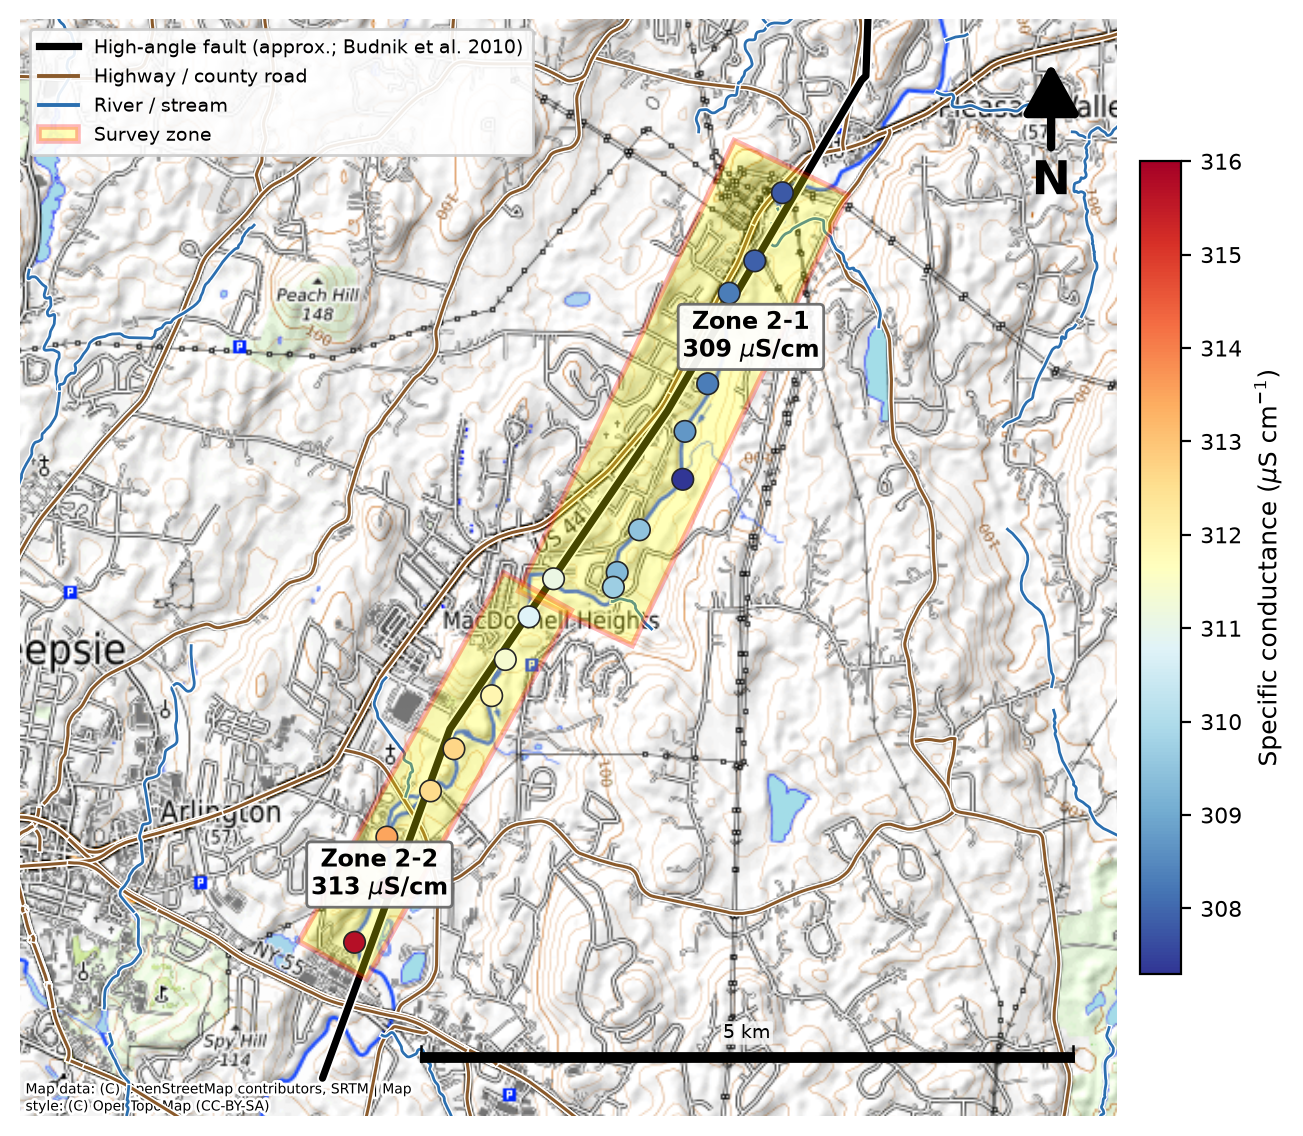
\includegraphics[width=0.52\linewidth]{figures/site2.png}
	\caption{Site 2, symbolised as in Figure~\ref{fig:site1}: terrain base, roads (brown) and streams (blue), survey points coloured by specific conductance, and red-outlined survey zones labelled with their mean specific conductance. Zones are numbered in ascending order downstream. High-angle faults (thick black) are approximate, digitized from \citet{budnik2010}. Statistical comparisons between zones are given in Table~\ref{tab:ttest}.}
	\label{fig:site2}
\end{figure}

Site 3 (Figure~\ref{fig:site3}) contains four zones (Zones 3-1, 3-2, 3-3, and 3-4), with the zone transitions corresponding to a side stream (Contrast C) and two faults (Contrast D and E). The east fork of Wappinger Creek intersects a small side stream, turns river left at a fault intersection, then wraps around a hill and darts river left along a second fault line. Zones 3-1 and 3-2 yielded mean specific conductance levels of 359.8 and 350.6~$\mu$S/cm respectively, while Zones 3-3 and 3-4 had mean values of 342.4 and 360.4~$\mu$S/cm respectively. We collected data for Site 3 over two days, but this does not affect the contrasts reported here, because every zone-to-zone comparison was computed within a single day's data collected sequentially along the reach. Specific conductance decreased after the tributary junction (Contrast C) and after the first fault crossing (Contrast D), then increased sharply after the second fault crossing (Contrast E, Figure~\ref{fig:site3}); as detailed below, only the increase at Contrast E reached statistical significance. The three transitions at Site 3 separate cleanly by feature type. The tributary junction (Contrast C) dilutes the main stem, consistent with lower-conductance side-stream input; the first fault crossing (Contrast D) carries the least statistical power of the survey and sits immediately downstream of that dilution, and its small decrease is not significant; and the second fault crossing (Contrast E) produces the largest step of the entire study, an 18.0~$\mu$S/cm rise significant at $p < 0.001$. The spatial coincidence of the strongest increase with a mapped fault, and its absence at the tributary, is the core observation the statistics support.

\begin{figure}[htbp]
	\centering
	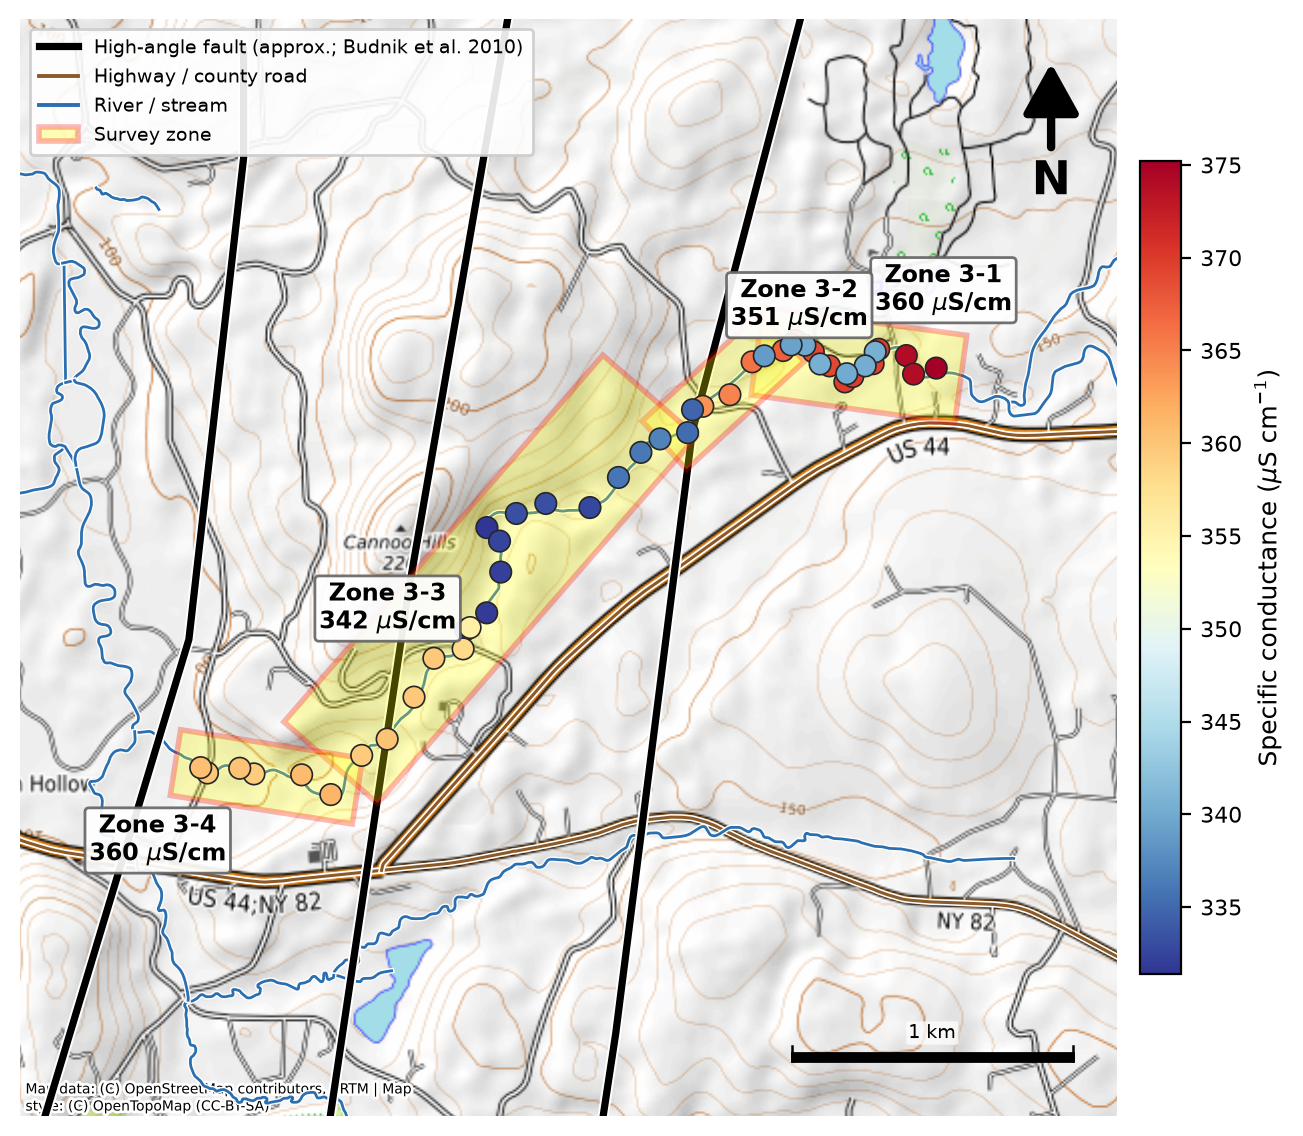
\includegraphics[width=0.85\linewidth]{figures/site3.png}
	\caption{Site 3, symbolised as in Figure~\ref{fig:site1}: terrain base, roads (brown) and streams (blue), survey points coloured by specific conductance, and red-outlined survey zones labelled with their mean specific conductance. Zones are numbered in ascending order downstream. High-angle faults (thick black) are approximate, digitized from \citet{budnik2010}. Across the fault crossing between Zones 3-3 and 3-4 the mean specific conductance increases sharply, whereas the tributary junction and the weaker fault crossing show little change; statistical comparisons are given in Table~\ref{tab:ttest}.}
	\label{fig:site3}
\end{figure}

Chloride sampling showed chloride measurements consistent with the long-term studies shown by Kelly et al. 2019 \citep{kelly2019} (Figure~\ref{fig:chloride}). Strong contrasts in chloride occurred close to where the geological fault line exists with concentration peaking $\sim$1000 meters upstream of the long-term study point. Because this transect was collected in summer, nearly two years after the conductivity survey, its agreement with the Contrast E crossing corroborates the specific-conductance step with an independent ion, in an independent year, and under baseflow conditions when direct road-salt runoff is not occurring. The chloride peak thus reinforces the interpretation that groundwater discharging near the fault, rather than surface runoff, carries the elevated salt into this reach.

\begin{figure}[htbp]
	\centering
	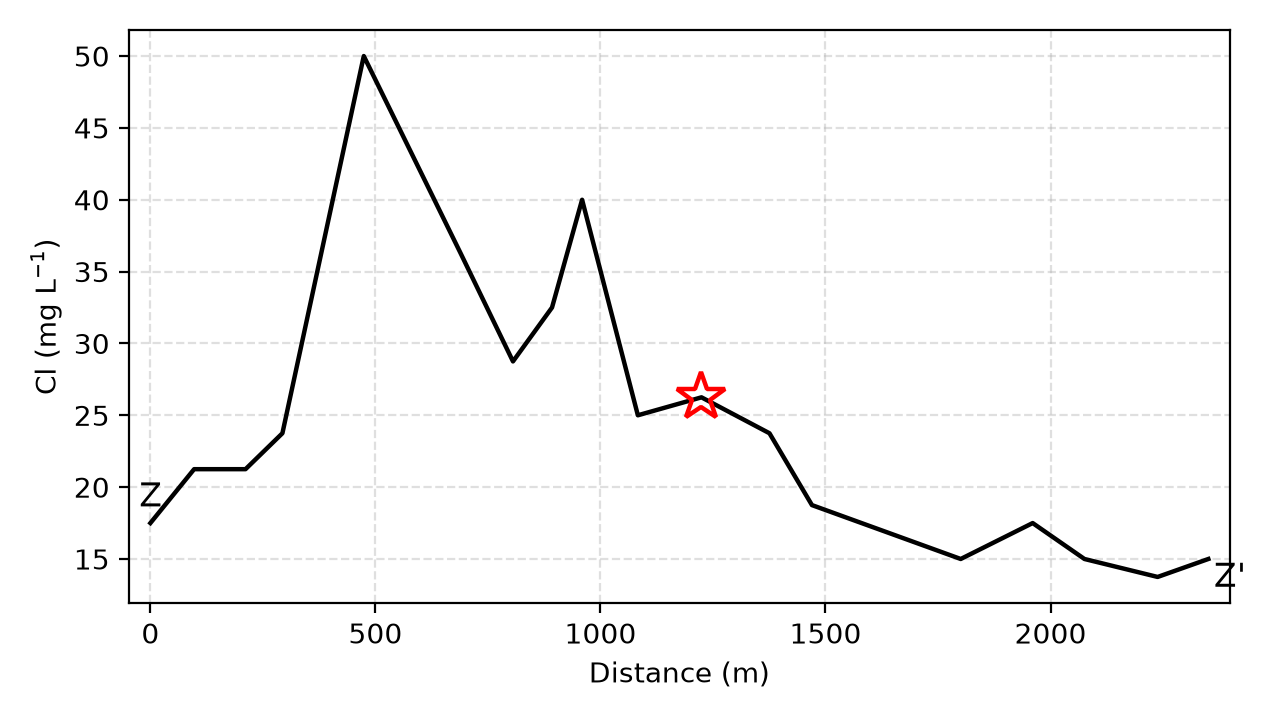
\includegraphics[width=0.71\linewidth]{figures/chloride.png}
	\caption{Chloride measurements along zones 3-3 and 3-4 shown in relative distance from points Z to Z'. The red star indicates the sampling point from the 32-year dataset introduced by Kelly et al. 2019 \citep{kelly2019}.}
	\label{fig:chloride}
\end{figure}

\subsection{Two-sample $t$-test}

Each contrast compares two adjacent reaches of Wappinger Creek separated by a geologic feature, tested with a two-sample Welch $t$-test on the raw specific-conductance measurements (Table~\ref{tab:ttest}). Here $\bar{x}_1$ and $\bar{x}_2$ are the upstream and downstream zone means ($\mu$S/cm), $n_1$ and $n_2$ their sample sizes, and the ``Boundary'' column records whether the separating feature is a mapped fault crossing or a tributary junction. At a significance threshold of $\alpha = 0.05$, the two fault crossings with the clearest geometry (Contrasts B and E) show significant increases in specific conductance ($p < 0.001$); the third fault crossing (Contrast D) and the two tributary-confounded contrasts (A and C) do not reach significance. A nonparametric Mann--Whitney $U$ test gives the same picture for B, D, and E.

% Table auto-generated by src/stats.py from data/salinity-dataset.xlsx.
\begin{table}[htbp]
	\caption{Two-sample Welch $t$-test results for each upstream/downstream contrast. Contrasts B and E (fault crossings) are significant at $\alpha = 0.05$.}
	\centering
	% Auto-generated by src/stats.py -- do not edit by hand.
\begin{tabular}{cclccrrrc}
\toprule
Contrast & Zones & Boundary & $n_1$ & $n_2$ & $\bar{x}_1$ & $\bar{x}_2$ & Welch $t$ & $p$ \\
\midrule
A & 1-1, 1-2 & tributary & 4 & 5 & 259.9 & 259.4 & -1.35 & 0.264 \\
B & 2-1, 2-2 & fault & 10 & 8 & 308.8 & 313.1 & 5.63 & $<$0.001 \\
C & 3-1, 3-2 & tributary & 17 & 6 & 359.8 & 350.6 & -1.24 & 0.248 \\
D & 3-2, 3-3 & fault & 6 & 17 & 350.6 & 342.4 & -1.15 & 0.286 \\
E & 3-3, 3-4 & fault & 17 & 6 & 342.4 & 360.4 & 5.83 & $<$0.001 \\
\bottomrule
\end{tabular}

	\label{tab:ttest}
\end{table}

\section{Discussion}

\subsection{Contrasts}

Two contrasts showed statistically significant changes in specific conductance: Contrasts B and E, from Sites 2 and 3 respectively. Each is a fault crossing, and each showed a statistically significant increase in specific conductance after the fault line interaction at $\alpha$ = 0.05, indicating a likely increase in stream salinity. The tributary-confounded contrasts A and C both showed decreases in specific conductance that did not reach significance; in any case these do not bear on our main conclusion about faults, because each corresponded to the location of an active tributary inputting water to the main stem of the creek, and measurements at Site 1 were taken during a rain event that occurred during sampling that day. The salinity levels for this section of the creek were between 50--100~$\mu$S/cm lower than the measurements taken at the other two sites. At Contrast C the active tributary measured nearly 150~$\mu$S/cm lower than the specific conductance measurements at Zones 3-1 and 3-2.

Of the three fault crossings that do not coincide with an active tributary (Contrasts B, D, and E), two showed a statistically significant increase in specific conductance, while the third, Contrast D, did not reach significance at $\alpha$ = 0.05 (Welch $t$ = $-1.15$, $p$ = 0.286). We do not read the non-significant crossing as evidence against fault-mediated transport. Contrast D compares the two zones with the most unequal sample sizes ($n_1$ = 6, $n_2$ = 17; Table~\ref{tab:ttest}) and lies immediately downstream of the tributary-diluted Zone 3-2, so its two reaches begin from different baseline concentrations and the comparison carries the least statistical power of the five. A single non-significant crossing bounds the strength of any inference we can draw from three examples, but it does not weaken the significant increases at Contrasts B and E, each of which recovered a clear signal from the same small-sample setting. We therefore present these three crossings as an initial, spatially explicit example of the pattern rather than as a population-level test of it. Later additional observation of longitudinal chloride concentrations across Contrast E (Figure~\ref{fig:chloride}, Z to Z') indicated the same strong contrast associated spatially with mapped fault locations.

A published 32-year dataset \citep{kelly2019} from the same stream reach as our study (Figure~\ref{fig:site3}, star; Figure~\ref{fig:chloride}, Z to Z') indicated that stream chloride has gradually increased in the area from annual means of roughly 15~mg/l in the 1980s to over 40~mg/l for annual means by the 2010s. This increase through time, as well as other findings \citep{kelly2019}, suggest a strong tie to human applications of road salt in the region. The elevated levels in streamflow in summer strongly suggest artificially elevated chloride levels overall, well above geologic background levels in groundwater. However, this study used only one location of data collection for long-term work on the stream \citep{kelly2019}, and was therefore not able to look at the spatial aspect of possible fault controls as transport pathways for road salts, as we have here. This new spatial conductivity and chloride data (Figure~\ref{fig:chloride}), in combination with the findings of similar concentrations of chloride during this extensive long-term study in the same stream stretch \citep{kelly2019}, together offer a much stronger link to road salts and their spatial controls on transport from faults. Collectively, this provides strong initial evidence that linear fault zones are indeed aiding in the preferential input of salt-polluted groundwater into streams at locations that correspond to where these major km-scale geologic structures connect both streams and highways.

\subsection{Addressing possible alternative sources of salinity in Wappinger Creek}

Increases in salinity can also occur as salts naturally enter the environment through the geological weathering of rock surfaces \citep{nimiroski2002}. The bedrock below Wappinger Creek consists of metamorphosed clastic sedimentary rocks \citep{budnik2010} known to have minimal influence of stream salt input. A 2008 study of sodium chloride retention in the east branch of Wappinger Creek (a portion of our study site) identified average salt input to the stream from various sources such as road salt, parking area salt, sewage, or rock weathering. The result found road salt contributes to 83\% of stream salt input, while geological rock weathering accounts for only 1\% of the input \citep{kelly2008}. Therefore, we argue that rock weathering is likely a tiny portion of total stream salt input and cannot account for the inferred changes in salinity we observed along fault zones in our study. This local partitioning is consistent with the wider regional picture. Syntheses of the anthropogenic salt cycle attribute the accelerating mobilization and accumulation of salt in temperate watersheds to human activities, with road deicing prominent among them \citep{kaushal2023saltcycle}, and mass-balance work across a comparable metropolitan region shows that a large fraction of applied road salt is retained in, and only slowly released from, groundwater rather than flushed directly to streams \citep{vanmeter2024}. Both lines of evidence point to a mobile, human-derived chloride pool held in the subsurface, precisely the pool that a conductive fault could route preferentially toward the channel. The elevated summer conductivities we recorded, at a time of year when direct road-salt runoff is absent, are difficult to reconcile with a purely geologic source and instead implicate this stored anthropogenic salt. Stream salinity can also rise near developed land from inputs unrelated to faults or highways, such as residential runoff and lawn or agricultural fertilizers. Because our sampling took place entirely within conserved forest, managed under a single entity with no fertilization practices, we can discount fertilizer runoff as a driver of the contrasts we observed.

\subsection{Placing fault-mediated transport within the freshwater salinization syndrome}

The gradual, sustained salinization of temperate freshwaters is now commonly described as a freshwater salinization syndrome, a coupled set of physical, chemical, and biological changes driven by the accumulation of anthropogenic salts \citep{kaushal2023factors,dugan2023}. Kaushal and coauthors organize the controls on this syndrome into a small set of state factors, among them the geology of a watershed and the flowpaths that connect salt sources to receiving waters \citep{kaushal2023factors}. Our results speak directly to the intersection of those two factors. Rather than treating the subsurface as a uniform reservoir that releases stored road salt diffusely, we find that a specific geologic structure, the high-angle fault, appears to organize where that release reaches the stream. This is mechanistically plausible. Fault zones are well documented to act as high-permeability conduits, or, where mineralized and sealed, as barriers, that focus groundwater flow \citep{bense2008,ferrill2025}, and recent three-dimensional modeling shows that the hydraulic-conductivity contrast between a fault and the surrounding rock can control how recharge is partitioned and where groundwater discharges to the surface \citep{marti2025}. Viewed through the syndrome framework, a fault is not a separate salt source but a flowpath that concentrates an existing anthropogenic source at discrete points along a channel. This distinction matters for consequences as much as for causes, because chloride delivered to a stream in such a focused way can raise local concentrations toward levels shown to restructure freshwater plankton communities \citep{greco2023}, and to act together with warming to compound those community-level effects \citep{mcclymont2023}.

\subsection{Suggestions for future research}

More investigations are needed in the coming years to better understand this newly observed process of salt movement through groundwater from road to stream along geologic faults. Additional sampling in bodies of water where major fault lines are present is required to concretely determine to what extent fault lines are adding saltier groundwater into streams in other regions globally. This sampling technique needs to be replicated at greater spatial scales to come to a more comprehensive conclusion regarding the prevalence of faults in contributing to the movement of road salts from highways through groundwater, particularly in regions with different lithologies and tectonic history. Our evidence has shown that of these three case examples of highway-fault-stream connections that we could isolate, all three point to a potential link between pre-existing fault lines and hint at the processes by which stream salinity levels are increasing, but additional research could further strengthen these findings. Beyond broader spatial replication, several targeted methods could test the transport mechanism itself more directly. Paired groundwater and surface-water sampling at fault crossings, combined with environmental age tracers, would establish whether the water discharging near a fault is older, deeper groundwater rather than recent local runoff, an approach already used to infer fault hydrology from apparent groundwater ages along bore transects \citep{cook2022}. Chloride-to-bromide ratios could further fingerprint deicer-derived salt against geologic end-members, and repeating the survey across contrasting lithologies and tectonic settings would show how far the pattern generalizes.

\subsection{Management implications of conclusions}

Salt input to streams, rivers, and lakes through groundwater input will continue, even if the use of road salts ceases due to the long transit time of water in groundwater flow systems \citep{perera2013}. This is concerning for human and aquatic life. Mitigation options to reduce road salt contamination could involve alternative or spatially unique methods to de-ice roads \citep{willmert2018}. Roads should not be treated as homogeneous due to the differences in vegetation and biome around them and unique geologic structures below them, and prior to treatment, mitigation of road salt impacts to the environment should be further taken into account \citep{ledford2016}.

Although road salts are cost-effective, their true cost is higher than similar de-icing agents due to its environmental cost \citep{kelting2010}. There exist various de-icing agents and methods that pose less of a threat to the environment such as anti-icing and pre-wetting \citep{ramakrishna2005,kelly2019}. To aid in reducing the negative impacts of road salts, small and large local governments could develop a salt management plan, as well as effectively train staff and local populations about the harmful effects of road salts and how to monitor for their impacts \citep{kelting2010}. The first step in a salt management plan is to identify salt sensitive areas, such as groundwater recharge areas, wetlands, shallow water tables, drinking water sources, salt-sensitive vegetation. With these new findings outlined here, we argue that known geologic information on locations of high-angle faults should also be included. Based on these different sets of geographic information, the salt management plan outlines steps to use another different de-icing agent if a road section intersects any known fault zones. Such geologically informed targeting complements, rather than replaces, the broader operational practices now being formalized at the state level. In New York, the Adirondack Road Salt Reduction Task Force has recommended a coordinated program of application-rate reductions, calibrated and pre-wetting equipment, brine-based anti-icing, and staff training \citep{adirondack2023}, measures that lower the total salt load entering the subsurface everywhere. Our findings suggest that where such programs must prioritize limited resources, road segments that cross mapped fault zones are logical candidates for the earliest and most aggressive reductions, because the salt applied there has a direct structural pathway to nearby streams.

\section{Conclusions}

We set out to test whether high-angle geologic faults act as preferential pathways that route road-salt-contaminated groundwater from highways into streams, using three fault-crossing reaches of Wappinger Creek as a spatially explicit case study. Applying a two-sample Welch $t$-test to reach-scale specific-conductance surveys, we found that two of the three fault crossings not confounded by an active tributary showed statistically significant increases in stream salinity across the structure ($p < 0.001$), while the third did not reach significance in the comparison with the least statistical power. A later longitudinal chloride survey reproduced the strongest of these steps at the same mapped fault location, and a published 32-year record from the same reach independently ties the elevated, summer-persistent salinity to decades of anthropogenic road-salt application rather than to geologic weathering. Taken together, these observations provide initial, spatially resolved evidence that faults can concentrate an existing anthropogenic salt pool at discrete points along a channel, placing this mechanism at the intersection of the geology and flowpath state factors of the freshwater salinization syndrome. Because our conclusions rest on three crossings within a single lithology, we present them as an illustrative example rather than a definitive population-level test, and we have outlined age-tracer, ionic-ratio, and multi-lithology studies that could test the mechanism more directly. If the pattern holds more broadly, it carries a concrete management implication: mapped fault locations are readily available geologic information that could help target salt-reduction efforts toward the road segments where contaminated groundwater has the most direct route to surface water.

Two broader points follow. Methodologically, matching the statistical test to the structure of the data matters here: a two-sample Welch test, which accommodates the unequal variances and unequal sample sizes of our zones, concentrates significance at the unconfounded fault crossings rather than spreading it across tributary junctions, and pairing it with a distribution-free check guards against over-interpreting the smaller contrasts. Substantively, because high-angle fault maps already exist for many regions, much of the geologic information needed to flag at-risk reaches is already in hand, and fault traces could be adopted as a planning layer wherever highways and salt-sensitive streams share a faulted catchment. Confirming how widely the mechanism operates will require the multi-site, multi-lithology sampling outlined above, but the case presented here establishes both the pattern and a practical way to search for it elsewhere.

\section*{Acknowledgements}

We would like to thank Marist University for providing funding and equipment to carry out our research as part of the first author's senior honors thesis and John Kittredge for collecting the data for the Chloride samples within Figure~\ref{fig:chloride}. We also would like to the Cary Institute of Ecosystem Studies for allowing us access to walk sections of the east-fork of Wappinger Creek which fall under their property line.

\section*{Conflict of interest}

The authors declare that they have no conflict of interest.

\section*{Data Availability}

Both the data, and the code, to reproduce figures and statistics from this paper are made available at the following GitHub Repository: \url{https://github.com/taddyb/wappingers_road_salts}

\bibliographystyle{unsrtnat}
\bibliography{references}

\end{document}
